\chapter{Introduction}
\label{Ch_Chapter1}

\section{Introduction}

In a real retrieval application (e.g.,Web search), the retrieval results using the initial query given by the user may not be satisfactory to the user; often, the user would need to revise the query to improve the retrieval/ranking accuracy. For some information seeking activities, the user may modify his query several times for one information need. In such an interactive retrieval scenario, the information available to us is more than just the current user query and the collection of documents. This paper summaries a set of experiments with term weighting for documents, using the measurement of term importance within an entire document collection. Then taking query it finds the relevant documents, if it exists then score the documents and sorting the scores it finds out the ranked documents. It is efficient while searching any document suppose in google users write the word or sentence that is called query, our proposed process will compute the importance of  word and rank the documents sequentially which were in maximum times in documents.

\section{Background and Present State of the Problem}

Bangla document ranking is an important aspect but no such research work had done on bangla language. Various methods and techniques have implied to rank documents of different country of different languages. In \cite{harman1986experimental} Donna Harman showed the importance of a term within the entire document collection has found, then number of term matches between a query and a document, they used two functions 1)the raw frequency and 2)the  log2  of frequency. Then doing normalization for document length they combined the measures and rank the documents. In \cite{lee1997document}Kent E.Seamons and Dik Lun Lee, they used term frequency and inverse term frequency, they compute the document ranking performance using precision and recall. In \cite{carbonell1998use} Xuehua Shen and ChengXiang Zhai, they used MMR method for ranking documents.
I have mentioned earlier, no research work yet not performed on bangle.  As there are several techniques for document ranking is present, these have their own limitations. One of the big problem of these systems is the accuracy is 	not better. If we need to implement these systems in real time purpose, the accuracy should increase otherwise it will be inefficient. So, I tried to increase the accuracy.


\section{Motivation and Aims}

Today the field of natural language processing(NLP) is increasing. As a nation, we have the historical background of language movement, which reminds us that everyone has the right to communicate using their own language. The growth in electronically available documents makes research and applications in automatic document ranking more and more important. Huge number of available documents in digital media makes it difficult to obtain the necessary information related to the needs of a user. In order to solve this issue, document ranking system can be used. Many work have done in various languages in different countries but there is no previous works in bangla on the basis of document ranking. It encourages me to do the work on bangla document ranking. Now my aim is to identify the document on the basis of importance of words in bangla so that while doing web search user can see the ranked document corresponding their given query. By using the ranking process, a user can decide if a document is related to his/her needs without reading whole document.
Document ranking systems can be categorized as extractive or abstractive according to the way the ranking is created. In extractive ranking approaches, the goals are identifying most important concepts in the input and giving relevant documents found in the document set as an output.
In abstractive ranking approaches, first the system understands the texts and then it creates ranking with its own words. The abstractive ranking is similar to the way a person creates ranking. Abstractive ranking remains as a difficult task in natural language processing.



\section{Objectives and Specific aims}

From the above discussion it is found that bangla document ranking is an important thing in our country while reading any bangla documents or newspapers. The objectives of my research are to identify the relevant documents within the given user query.
And the specific aim is to rank relevant document with corresponding query. The query is matched word by word in relevant documents and ranked documents with cosine similarity.

\section{What is NLP \& Document Ranking?}

Natural Language Processing, NLP is a branch of artificial intelligence that deals with analyzing, understanding and generating the languages that humans use naturally in order to interface with computers in both written and spoken contexts using natural human languages instead of computer languages.

\subsection{Document Ranking}

Document ranking is the process of ranking documents with document and query.

\begin{figure*}[htp]
	\centering
		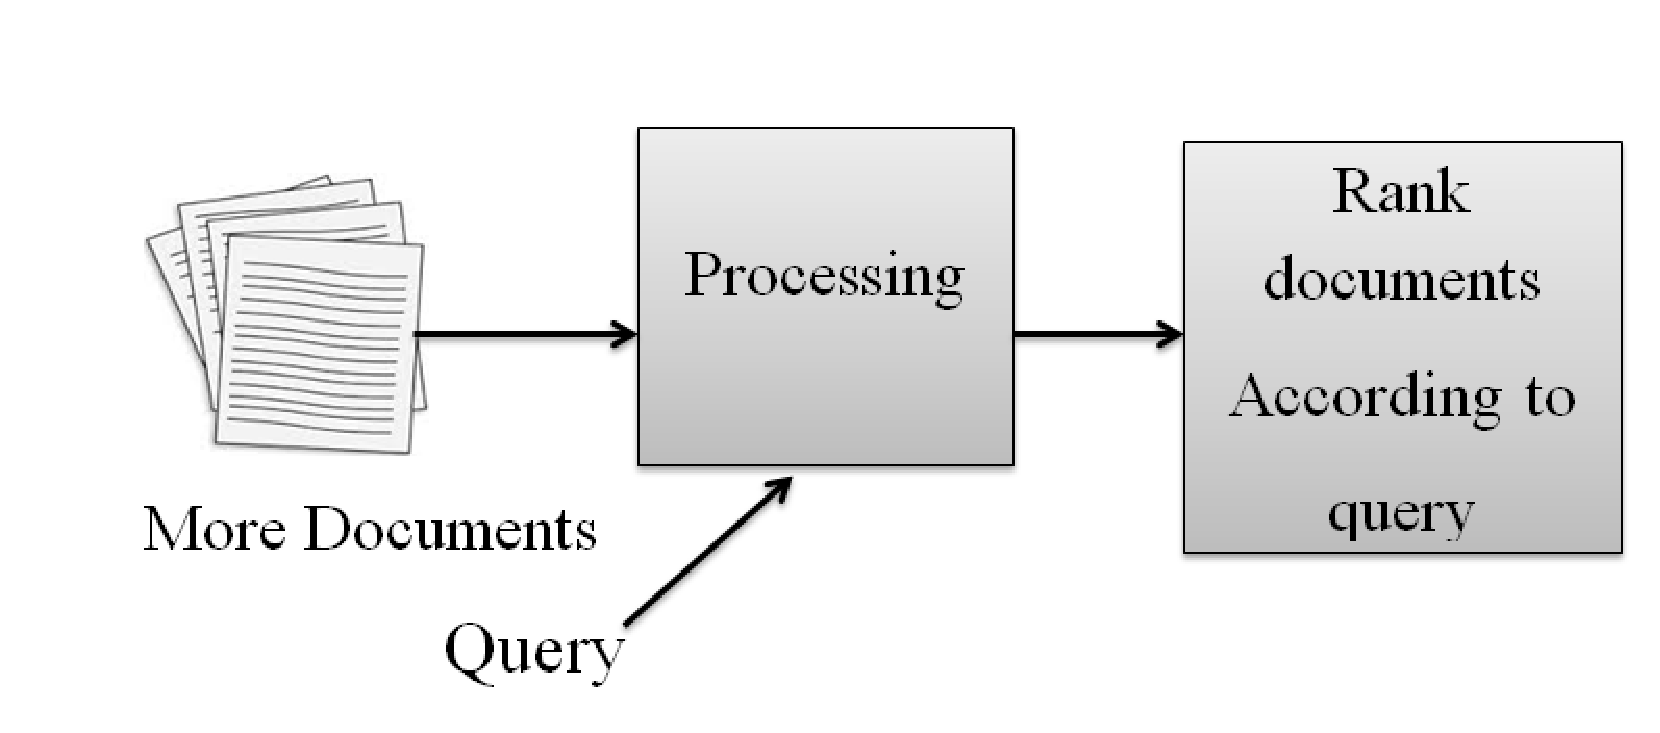
\includegraphics[width=.65\textwidth]{figure/one.eps}
	\caption{Main Process of our system}
	\label{Figure:process}
\end{figure*}





\section{Organization of the Thesis}
%
The dissertation is organized as follows: 

\begin{itemize}

\item \textbf{Chapter 1 Introduction.} In this chapter we have already discussed bangla document ranking, previous works in this field, motivation , objectives and aim of our thesis. Actually it is the preliminary chapter which describes the basic idea about the project. 

\item \textbf{Chapter 2 Literature Review.} It contains the sufficient description about my thesis topic. Definition of various terms, mathematical background, technology that we have applied for implementing our work. 

\item \textbf{Chapter 3 Proposed System.} It representing the whole process of our system, each part of our system that we have applied in our system.  

\item \textbf{Chapter 4 Implementation.} The chapter named implementation process encloses  the  procedure  of  the  method  implementation.

\item \textbf{Chapter 5 Experimental Results and Discussion.} This chapter contains the experimental set up and some experimental results that have been done during implementation of the method. We try to represent the performance analysis here.

\item \textbf{Chapter 6 Conclusion and Future Scopes.} This chapter concludes our thesis work mentioning the goal that we are achieved in by completing our work. We also mention the correctness and accuracy of our methodology by which we have done the work.

\end{itemize} 
%
